% !TeX root = ../thuthesis-example.tex

\chapter{卷积神经网络的分层抽象特性和遗忘方法}
上一章阐述了遗忘学习的研究现状和面临的主要挑战。本章的主要内容是介绍卷积神经网络的一个重要特性,即分层抽象特性。为了让读者能够更好地理解卷积神经网络的分层抽象特性,我们将首先介绍卷积神经网络的工作原理以及其中较为深层的设计思想。接下来我们会正式定义机器学习遗忘的概念,再介绍基于卷积神经网络分层抽象特性的遗忘思想。最后将介绍评价遗忘的性能指标。

\section{卷积神经网络的介绍}

\subsection{卷积神经网络的结构}
\paragraph{}首先,我们看卷积神经网络的网络结构,大致了解卷积神经网络的框架。卷积神经网络和多层感知机的神经网络很类似,它们都可以通过像堆积木一样来组装构建。然而,卷积神经网络里和多层感知机不同的是出现了Convolution 层(通常称为卷积层)和Pooling 层(通常称为池化层)。
\paragraph{}下一小节会详细介绍卷积层与池化层,在这我们首先看如何将各层组织起来构建卷积神经网络。基于多层感知机的神经网络中,相邻层的各个神经元之间都有连接,这样的结构被称为fully-connected(通常称为全连接)。Pytorch工具中已经实现了全连接层。如果使用全连接层来搭建网络,我们可以通过如图\ref{fig:chapter3_3}所示的神经网络结构实现一个五层的简单神经网络。
如图\ref{fig:chapter3_3}所示,在使用全连接层搭建的神经网络中,全连接层后面直接跟着激活函数ReLU(或者Sigmoid)。这里使用了4 层全连接和ReLU的组合,接着的第5层是全连接层,最后一层则是Softmax层,输出最终的预测结果。
\begin{figure}
    \centering
    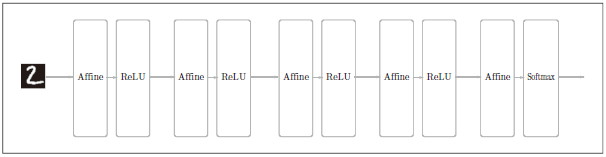
\includegraphics[width=0.9\linewidth]{chapter3_3.png}
    \caption{全连接网络结构示意图}
    \label{fig:chapter3_3}
\end{figure}
如图\ref{fig:chapter3_2}所示,这就是一个卷积神经网络的例子。
\begin{figure}
    \centering
    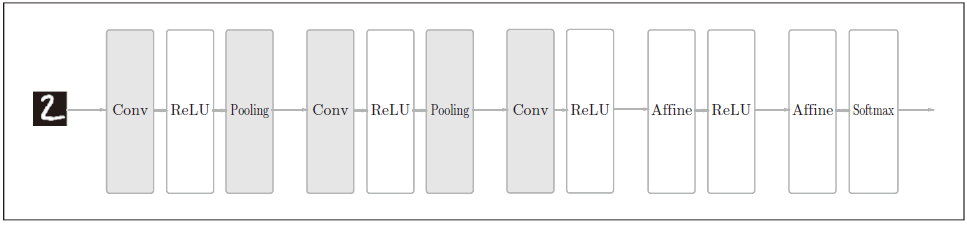
\includegraphics[width=0.9\linewidth]{chapter3_2.png}
    \caption{卷积神经网络结构示意图}
    \label{fig:chapter3_2}
\end{figure}
如图\ref{fig:chapter3_2}所示,卷积神经网络中增加了卷积层和池化层。卷积神经网络的单个层连接的顺序是卷积层,激活函数层和池化层,其中池化层有时可以省略。这样的组合方式可以被理解为前面的全连接层和激活函数层组合连接被替换成了卷积层,激活函数层和池化层的连接。另外,在如图所示的卷积神经网络中,靠近后面的输出层中使用了全连接层和激活函数层ReLU组合。然后,最终的输出层中则使用了全连接层和Softmax的组合。这样的搭配一般都是卷积神经网络中较为常见的搭配结构。
\subsection{卷积神经网络的原理}
\paragraph{}在全连接的神经网络中,各个层次都是通过全连接层来组织起来的。在全连接的层次中,各个神经元都是连接在一起的,全连接的网络的输出数量是可以任意指定的,没有数量上的限制。
\paragraph{}这样的结构会带来一定的问题,那就是数据的形状特征没有被充分地利用起来。用图片来举例,神经网络输入图片时,图片数据的格式一般是长、宽和高。长和宽代表图片像素点的长度和宽度,高代表图片采样通道的宽度。然而,这样的数据结构输入到全连接层搭建的神经网络中时,就会被拉长为一维的数据。举例说明,MNIST的数据集中一张图片的长是28个像素点,宽是28个像素点,高度是1个通道(图片用黑白表示)。这样的形状输入到全连接的网络中前会被展开成一列,就是784个数据点输入到网络中。按照常识可以知道,图片一般是三维的形状。
\paragraph{}这样的形状结构中包含重要的空间位置关系信息。比如通道与通道之间的关联信息,空间上相互距离比较接近的像素点一般具有相似的值,距离比较远的像素点一般没有关联,因此三维形状的数据中可能会蕴藏很多可以挖掘的特征模式。全是全连接层的神经网络就会把数据拉长成一维数据,从而没有充分利用图片中的空间位置信息。
\paragraph{}卷积神经网络就不会这样,图片输入到网络中就是以三维数据的格式输入,一个卷积层处理好数据以后,让然会以三维的格式输入到下一个卷积层中。所以,卷积神经网络对于理解图像这样带有空间位置信息的数据是很有优势的。
\subsubsection{卷积层}
卷积运算发生在卷积层,卷积运算的计算过程类似滤波处理过程。因此用于卷积运算的卷积核有时又被称为滤波器。常规的卷积运算如图\ref{fig:chapter3_4}所示。图中展示的便是一次二维卷积运算的过程。输入数据的尺寸是4乘4,卷积核的尺寸是3乘3,没有边界填充的情况下,最终输出结果的尺寸是2乘2。
\begin{figure}
    \centering
    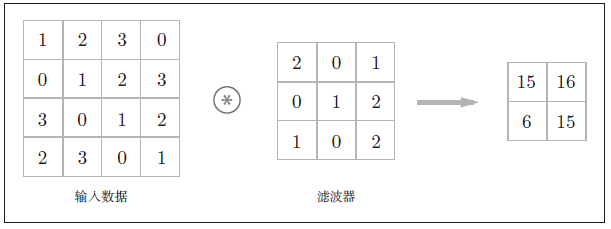
\includegraphics[width=0.9\linewidth]{chapter3_4.png}
    \caption{卷积神经网络结构示意图}
    \label{fig:chapter3_4}
\end{figure}
卷积运算的具体过程是什么样的呢?下面结合图片\ref{fig:chapter3_5}来具体说明。如图\ref{fig:chapter3_5}中的第一行所示,第一行灰色区域代表第一步卷积操作所发生的区域,这个区域内的数字和卷积核的形状是相同的,所以区域内的数字可以与卷积核中对应位置的数字相乘,然后再把这些相乘的结果相加就得到了第一个结果,运算后将结果保存到相应的位置。如图\ref{fig:chapter3_5}第二、三、四行所示将上面讲的过程在每个位置计算一遍,于是就完成了一次卷积运算。
\begin{figure}
    \centering
    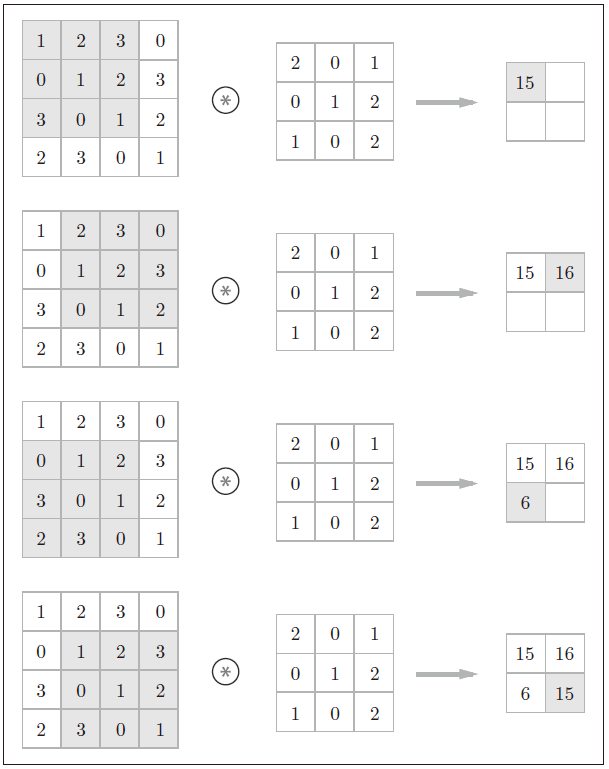
\includegraphics[width=0.9\linewidth]{chapter3_5.png}
    \caption{卷积神经网络结构示意图}
    \label{fig:chapter3_5}
\end{figure}
和全联接的网络相同,除了网络的权重之外,还有偏置。卷积神经网络中偏置的个数一般是卷积核的个数,而且每个卷积核对应的偏置的维度一般是1乘1。计算完卷积之后,在相应结果的每个位置再加上偏置数字便得到了最终输出的数据,其计算过程如图\ref{fig:chapter3_6}所示。对于输入数据,滤波器(维度是3*3)与输入数据(维度是4*4)进行卷积元算后便得到了初步的输出结果(维度是2*2),之后再将这个结果的每一个位置加上该卷积核对应的偏置数值,得到了最终结果(维度是2*2)。
\begin{figure}
    \centering
    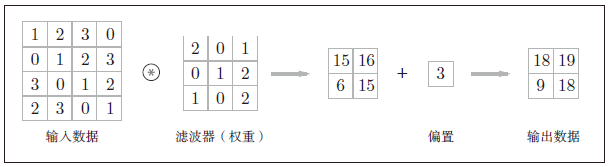
\includegraphics[width=0.9\linewidth]{chapter3_6.png}
    \caption{卷积神经网络结构示意图}
    \label{fig:chapter3_6}
\end{figure}
三位卷积运算与二维卷积运算不同的是,卷积核的维度从2维提高到了3维,除了有长和宽的信息,还有通道数的维度。如图\ref{fig:chapter3_7}所示,以3通道为例,其运算过程与二维相似,现将对应位置的数字相乘,然后将相乘之后的结果相加,便得到了输出结果。
\begin{figure}
    \centering
    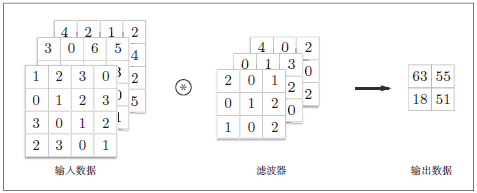
\includegraphics[width=0.9\linewidth]{chapter3_7.png}
    \caption{卷积神经网络结构示意图}
    \label{fig:chapter3_7}
\end{figure}
\subsubsection{池化层}
为了减少参数的数量,提高神经网络泛化能力,在卷积伸进网络进行卷积运算以后,通常会进行池化操作。池化操作会同时减少卷积操作结果的长度和宽度。其运算过程如图\ref{fig:chapter3_8}所示。在第一行,图中灰色区域就是池化操作的一个操作单元,这个操作单元的大小来自池化操作的输入参数。池化操作的输入是图中灰色区域内的数字,输出是一个数字。中间的运算过程一般有两个算法,一种是去所有数字中最大的数字,这种算法一般被称为最大池化操作;另外一种算法是取区域内所有数字的平均数,这种算法一般被称为平均池化操作。
\begin{figure}
    \centering
    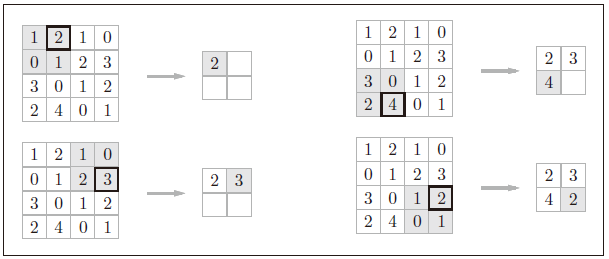
\includegraphics[width=0.9\linewidth]{chapter3_8.png}
    \caption{卷积神经网络结构示意图}
    \label{fig:chapter3_8}
\end{figure}
池化层与卷积层不一样的是,池化层没有训练参数,它的输入参数都是运算之前系统已经规定好的。池化层就是一个固定算法的函数。它另外一个特点是,池化操作后通道数是不变的,各通道是相互独立的,如图\ref{fig:chapter3_10}所示。
\begin{figure}
    \centering
    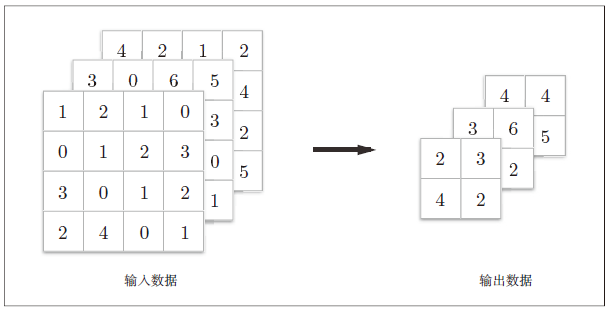
\includegraphics[width=0.9\linewidth]{chapter3_9.png}
    \caption{卷积神经网络结构示意图}
    \label{fig:chapter3_9}
\end{figure}
加入池化层后,神经网络对输入数据发生的一些微小干扰噪声具有很好的鲁棒性。如图\ref{fig:chapter3_10}所示,即使图片发生了微小偏移,经过池化操作后,其特征仍能被准确地识别出来。
\begin{figure}
    \centering
    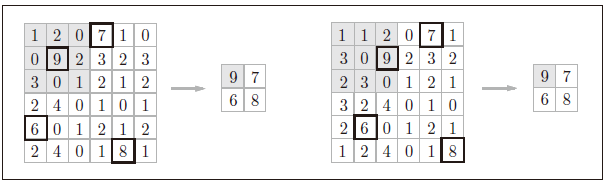
\includegraphics[width=0.9\linewidth]{chapter3_10.png}
    \caption{卷积神经网络结构示意图}
    \label{fig:chapter3_10}
\end{figure}
\section{卷积神经网络的分层抽象特性}
\subsection{人类视觉信息处理原理}
1981年来自美国的科学家David Hunter Hubel和来自瑞典的科学家Torsten Wiesel被授予了诺贝尔生理学或医学奖,以表彰他们研究人类视觉系统信息加工领域作出的杰出贡献。他们在人类视觉系统信息加工领域的工作贡献了当今神经生物学教科书视觉部分的一半内容,成为所有研究神经生物学方向学生的必学内容,这篇回忆录\cite{Hubel1998EarlyEO}中记录他们一起共事的过程。在他们的这篇工作\cite{https://doi.org/10.1113/jphysiol.1959.sp006308}中记录了麻醉后的猫的大脑对不同视觉光斑刺激的反应,并记录下了视觉皮层神经元的活动。
如图\ref{fig:chapter3_11}所示,他们在实验中发现,有一类细胞对一定范围视野内特定朝向上的刺激反应强烈,他们称这样的现象为朝向选择性,称这样的细胞为简单细胞。这样的细胞仅对狭窄的视觉感受野有反应,刺激他们最好的方式就是比较狭长的光斑,而且刺激的产生有明显的边界,当光斑覆盖整个作用区域时,并不能产生刺激反应。因此这样的细胞被看作是专门用来感受线条或边缘的信号接收器。他们通过进一步的实验发现,还有一类细胞,虽然对特定方向光斑的刺激有强烈反应,但是并没有明显的感受野。他们发现这样的细胞的上游是许多简单细胞,接受简单细胞发过来的刺激信号。他们称这样的细胞为复杂细胞。这种模式可以理解为复杂细胞是简单细胞的抽象,猫的视觉系统具有层级结构,图\ref{fig:chapter3_12}展示了简单细胞和复杂细胞的关系。
\begin{figure}
    \centering
    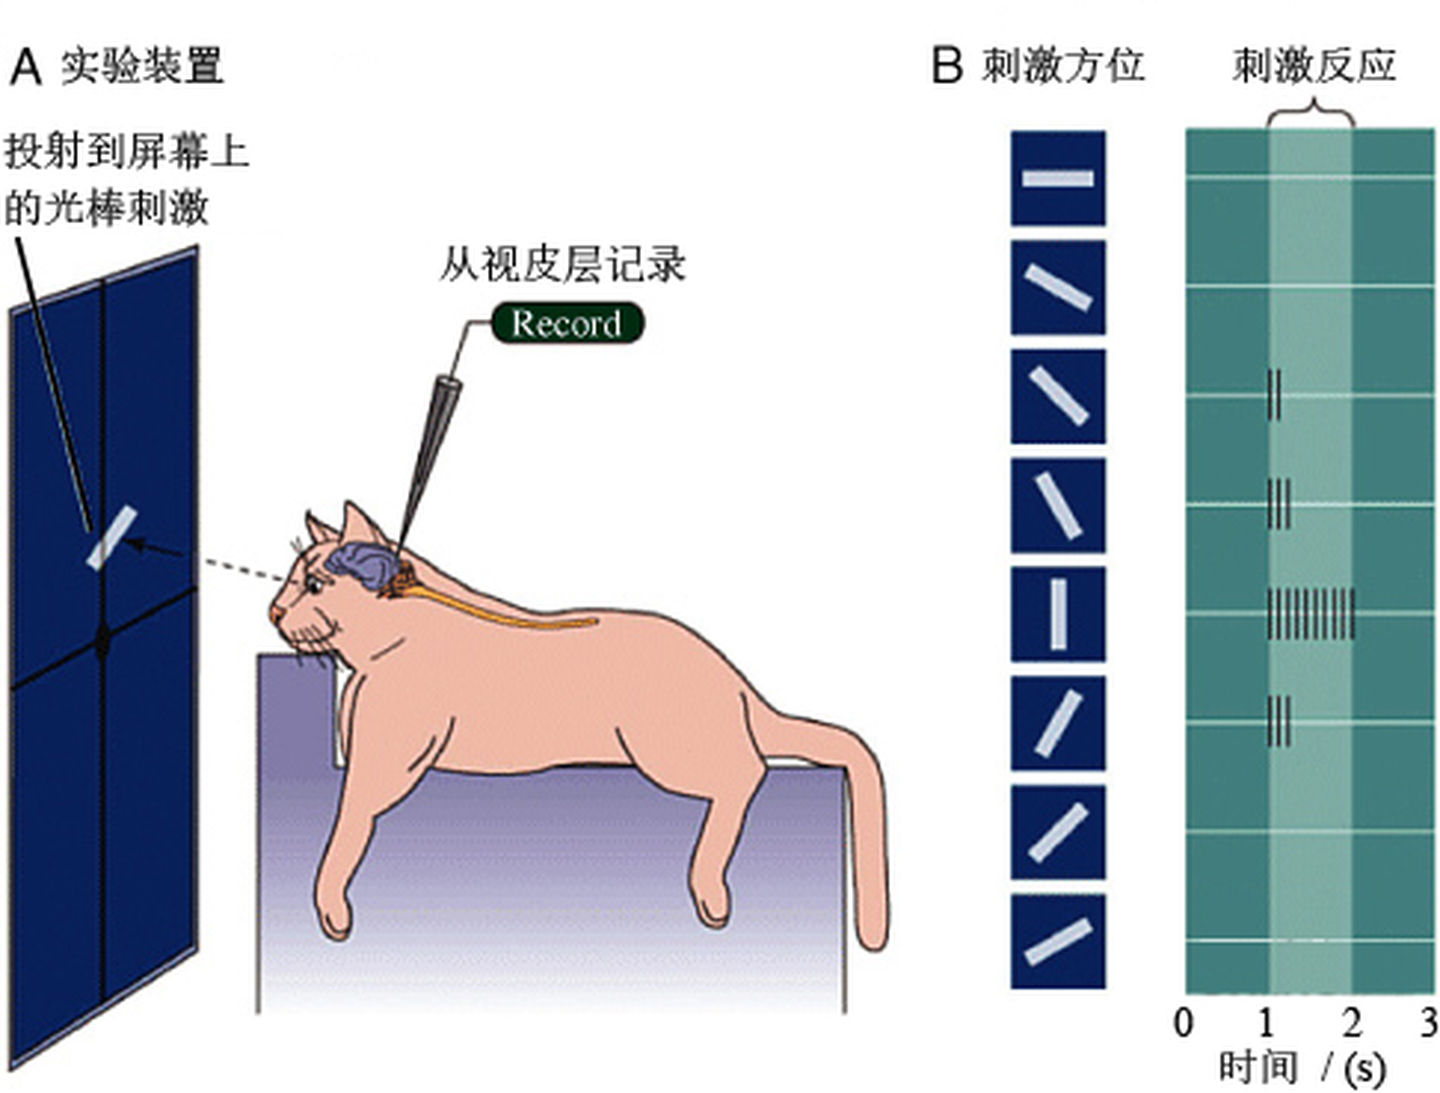
\includegraphics[width=0.9\linewidth]{chapter3_11.jpeg}
    \caption{人类视觉处理信息流程示意图}
    \label{fig:chapter3_11}
\end{figure}
他们这样的发现对理解人类视觉信息加工过程很有帮助。首先人类的视网膜接收外界传入的信号,经过简单细胞处理后,简单细胞完成了一些初级特征的提取,比如简单的直线或边缘的信息。简单细胞后面有复杂细胞,复杂细胞负责完成更为抽象层次信号的处理,比如由各种方向的直线或边缘组成的形状的信息,比如三角形或正方形等。复杂细胞上面的细胞负责处理更为抽象的信息,经过一系列信息的抽象后,人类大脑就能识别看到的图像是一个什么物体。因此人类视觉信息加工是一个不断将信号进行抽象处理的过程。(图片引自https://zhuanlan.zhihu.com/p/29853731)
\begin{figure}
    \centering
    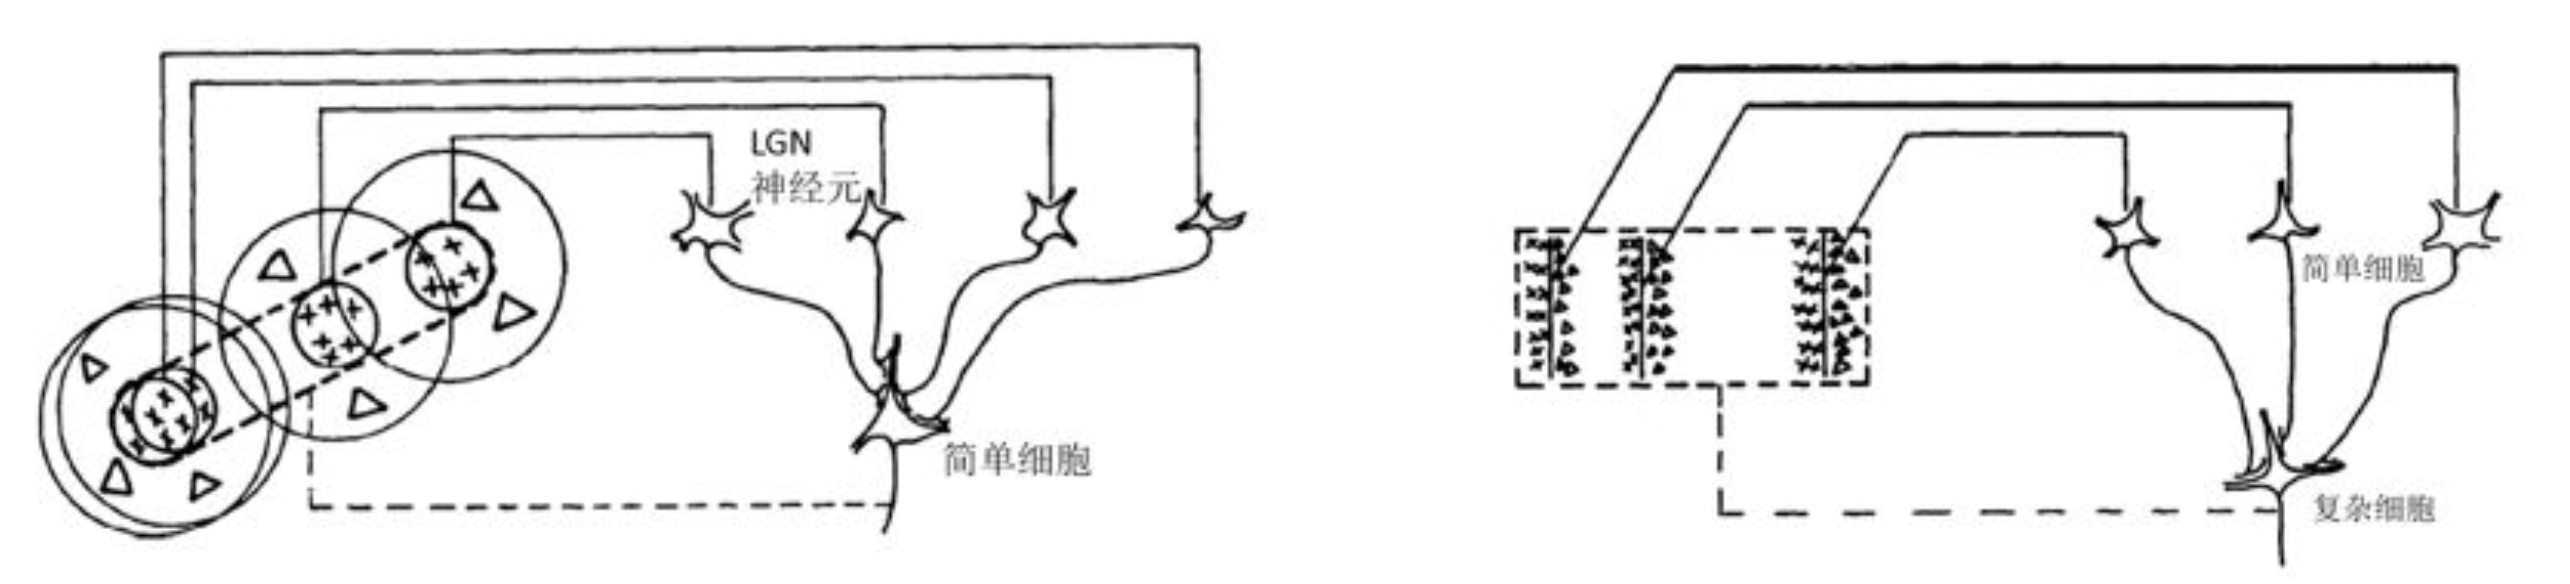
\includegraphics[width=0.9\linewidth]{chapter3_12.png}
    \caption{人类视觉处理信息流程示意图}
    \label{fig:chapter3_12}
\end{figure}

\subsection{卷积神经网络的分层抽象特性}
在这篇文章\cite{2019arXiv190906161K}中,作者提到了卷积神经网络是最接近还原人类视觉信息加工原理的人工神经网络。从本章第一节讲到的卷积神经网络的基本原理中可以知道,卷积神经网络中的卷积核在与输入数据进行卷积操作时,很类似人类视觉感受野中的朝向选择性。随着输入数据在多层卷积层中逐层传递,使得一些特征信息逐渐被卷积核提取,提取的信息也逐步抽象。本文将卷积神经网络这种区别于其他人工神经网络的特性称为卷积神经网络的分层抽象特性,层数较低的卷积核提取的是较为初级的基本特征,层数越高的卷积核提取的特征越抽象。如图\ref{fig:chapter3_13}所示, 图中上半部分展示了一个优化完成的8层卷积神经网络结构。下半部分则是参数渲染后的效果。我们可以看到第一个卷积层学到的信息是一些基础的信息,例如边和角;第三层学到了由边和角构成的图案;第五层则学到了由图案构成的物体的某个部分;最后,全连接层学到的是整个物体本身。由此可以看出在卷积神经网络模型中,越靠后面的层次往往是前面层次的抽象(这里我们称离输入端较近的层次为前面层次,离输入端较远的层次为后面层次),这种现象就解释了我们所说的分层抽象特性。
\begin{figure}
    \centering
    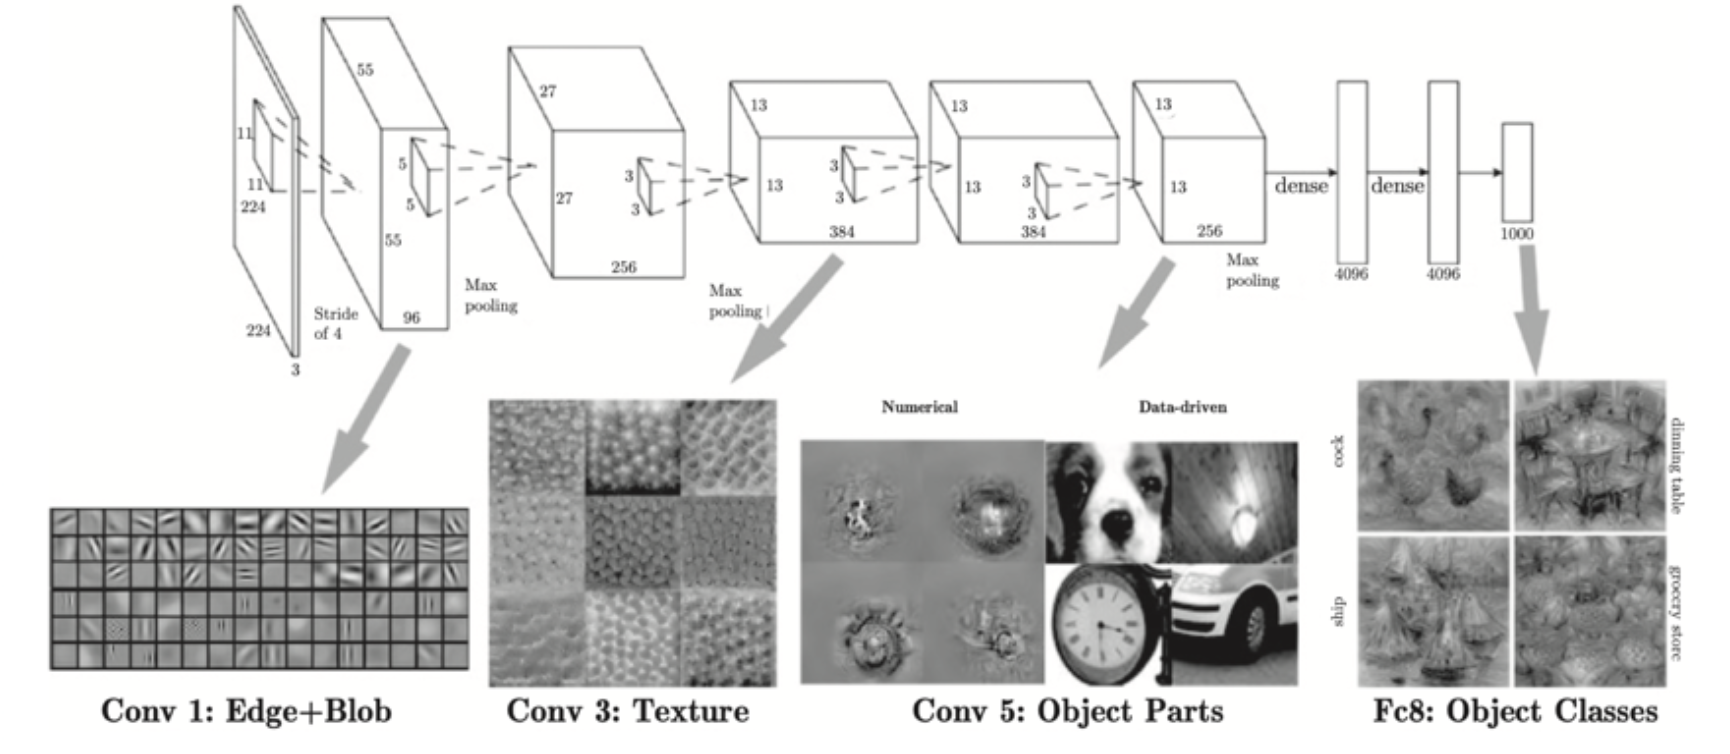
\includegraphics[width=0.9\linewidth]{chapter3_13.png}
    \caption{人类视觉处理信息流程示意图}
    \label{fig:chapter3_13}
\end{figure}

\section{基于卷积神经网络的遗忘方法}
\subsection{遗忘方法的思路介绍}
我们首先来讨论什么是遗忘。理想的遗忘效果是就好像一个神经网络模型从来没有使用遗忘数据训练过一样。换一个角度考虑,一个用户之所以会选择让模型遗忘自己的数据,其初衷是出于保护个人隐私。因此遗忘的目的就是为了防止模型攻击造成信息泄露当前的攻击方法有多种多样,我们无法也不可能去针对每种攻击方法去设置防御方法。我们能做的就是消灭信息,换句话说,消灭的信息越多,攻击者得到的信息就越少。消灭信息的极限就是重新训练。然而重新训练的代价是十分巨大的,一个神经网络模型少则几千个参数,多则高达数亿参数,重新训练的代价是十分昂贵的。所以完全消灭所有信息看起来是不现实的。
那么有没有一种折衷方案,既可以消灭信息,又能不用重新训练付出那么多代价?答案是肯定的,那就是我们不用消灭所有的信息,只消除一部分抽象信息,一些基本的信息是分类无关的,攻击者即使拿到也没有用途。这就用到了卷积神经网络特有的分层抽象特性,像人类视觉信息处理过程一样,卷积神经网络较低层次的卷积层只提取了较为基本的视觉元素,比如边、角、简单的条纹等等。随着网络层次的提高,抽象程度逐渐提高,卷积核的感受野也逐步扩大,从而能提取到更为抽象的信息,比如一些有固定模式的组织,图案等。到卷积神经网络比较高的层次后,感受野进一步扩大,从而能提到跟分类息息相关的本质特征,比如不同人脸的区分,以及不同物体的区分,如猫和狗,飞机和卡车等。
想一想,一个攻击者最希望获得哪一部分的信息呢。毫无疑问是和分类有关的本质特征信息,而不是那些比较基本的边和角的信息。沿着这个思路,于是我们就想出了一个可以既可以消灭信息,又能不用全部参数参与训练的折衷方案,那就是消灭层数较高层次的参数。
消灭参数之后会带来一个问题,我们不仅消灭了要遗忘数据的较高层次的抽象信息,同时也消灭了没有被遗忘数据的较为重要的分类信息。为了解决这个问题,我们想到了用重新训练的方法。这里说的重新训练不是指要训练所有的网络参数,而是只训练我们前一步骤消灭的参数,目的是恢复那些没有被遗忘类别的高层次的信息。这一步骤我们的做法是使用没有被遗忘类别的训练数据去训练这一部分参数。
等待模型收敛之后,我们就可以得到消除了遗忘类别高层次抽象信息,同时保留了未被遗忘类别的分类信息。

\subsection{确定分层}
\paragraph{}前面小节讨论了遗忘方法的思路方案。随之而来的问题就是,我们需要要重置一定层数的网络参数,我们究竟要重置多少层呢?重置层数的多少直接影响了遗忘效果的好坏以及重新训练的时间,因此确定分层数量是本方法的一个重要环节。
\paragraph{}为了确定重置参数的层数,我们的研究思路是首先设计一个评价分层好坏的数学指标,这样既可以清晰地指导本方法后续使用的过程,又能为确定分层提供一个具有一定使用价值的评判标准。
\paragraph{}这个指标由上面介绍的四个指标处理后的数值加权相加得来,其计算方法如公式。
% \paragraph{}I_synthesize = w_acc * v_acc + w_time / v_time + w_distance / v_distance + w_inf_scs / v_inf_scs
\paragraph{}$I_synthesize$代表综合计算指标,这个指标的数值越大代表分层的效果就越好。它不是一个绝对指标,而是一个相对指标,即只能用作对比量。这个指标由四个部分组成,第一个部分是准确率评价部分,$w_acc$代表准确率评价部分的权重,$v_acc$代表准确率指标的数值。第二部分是收敛时间评价部分,$w_time$代表收敛时间评价部分的权重,$v_time$代表收敛时间指标的数值。第三部分是激活距离评价部分,$w_distance$代表激活距离评价部分的权重,$v_distance$代表激活距离指标的数值。第四部分是成员推断攻击成功率评价部分,$w_inf_scs$代表成员推断攻击成功率评价部分的权重,$v_inf_scs$代表成员推断攻击成功率指标的数值。
\paragraph{}有了上述确定分层的计算指标,我们就可以对分层方法进行评价。在本遗忘方法的使用过程中,应当在什么时间去进行分层呢?是在每次执行遗忘算法的时候都需要分层一次吗?答案是否定的,我们无需在每次遗忘时均评价一次分层效果。对同一个网络结构,同一套网络训练数据集,我们仅需在首次遗忘时进行分层效果的测试,在后续的遗忘训练时,只需要使用首次遗忘时使用的分层数即可。至于为什么是这样我们将在本文第五章具体讨论。

\subsection{重置并冻结参数}
\paragraph{}对于重置并冻结参数的原因,在本章一开始的本方法的思路来源中已经得到了解释,是为了更好地消灭待遗忘数据在原网络中的信息。对于重置和冻结参数,我们将它们分开进行解释。
对于重置参数,我们首先考虑到的问题是,将原来需要重置参数的层次删除后,补充什么参数进去,这涉及到参数初始化的过程,也是很重要的一步。关于参数初始化有很多相关的研究成果,为了避免研究方向走偏,本文尚未对参数初始化这一变量进行系统性地研究。
我们反过来看对参数应当如何初始化,如果初始化的参数不正当,又会给我们的研究带来很大的麻烦,比如使得模型无法收敛,或者无法达到全局最优等。为了防止这样的由于参数初始化不当而带来的问题,我们选取的策略是,保存模型初始化参数,当网络中某些层次需要重置参数时,我们将保存下来的相应层次的网络参数补充到需要重置参数的层次当中。这样做的一个出发点是,既然这个网络模型初始化参数能够使得网络达到收敛状态,就说明这个参数是一个较为合理的初始化参数,没有均值过大或过小,或方差过大或过小的异常情况。经过实验证明,这种做法具有一定的合理性,在实验中并未发现由于重置参数不当而带来的网络训练无法收敛的问题。
\paragraph{}对于冻结网络,我们需要关注的问题是冻结网络的必要性方面,即到底需不需要冻结网络。对于这个问题,前人已经有人做了一定的研究工作。
\paragraph{}在这篇文章\cite{yosinski_2014_NIPS}中,作者设置了对比实验。如图\ref{fig:transfer_learning_3}所示,图中的第一行和第四行与本文无关。图中的第二行代表一个8层的卷积神经网络使用训练集B进行训练,得到baseB。第三层代表将卷积神经网络的后五层参数重置,并且将前三层网络参数分别进行冻结实验和非冻结实验。冻结实验得到的网络参数称为BnB,非冻结实验得到的网络参数称为BnB+。其中n代表进行冻结和非冻结实验的网络层数。如图所示,图中将前三层网络参数进行了冻结和非冻结对比实验。因此得到的网络参数分别为B3B和B3B+,B3B是冻结参数得到的网络参数,B3B+是非冻结参数得到的网络参数。实验所用到的训练数据均为训练集B。
\paragraph{}实验结果如图所示,selffer BnB和selffer BnB+标记为冻结参数实验得到的测试准确率和非冻结参数实验得到的测试准确率。baseB代表原训练完成网络测试准确率的大小,在这里作为参照。图中的横轴代表参与冻结实验的网络层数,和n的定义相同。结果展示了在冻结和非冻结实验中,非冻结参数的训练结果普遍好于冻结参数的训练结果,比如4层和5层。冻结其他层数时,冻结参数与非冻结参数的准确率结果相差不大。
\paragraph{}是否冻结参数对本方法的最终效果影响较大。因为这不仅涉及到训练之后模型的准确率,也涉及到训练过程的收敛时间问题。上面的实验并没有涉及到收敛时间。为了探究是否需要冻结参数的问题,本文也设计了专门冻结参数与非冻结参数训练的对比实验。具体实验过程和结果将在本文第四章集中展示。

\subsection{训练网络}
\paragraph{}对于重新训练网络,使用的数据集是原来的数据集减去要遗忘类别的数据集。因为是原数据集和遗忘数据集的差集,为了便于表达,以下称之为保留集。重新训练网络的目的已经在前文有所说明。重置了一部分网络参数以后,所有的训练数据中涉及到的分类信息已经全被消灭掉了。此时网络攻击者通过网络输出来还原训练数据的信息几乎是不可嫩的。为了保证没有被遗忘的类别达到删除参数以前的效果,我们使用保留集对重置的参数进行一定程度的还原。
\paragraph{}在重新训练网络的过程中,待更新的参数数量对比完全重新训练的参数数量,少了冻结层次的参数,因此训练网络中不需要对冻结的参数去计算梯度和更新。因此从网络参数的收敛速度上看,应当是有一些减少。为了检验训练速度能够提升多少,我们设计了对比实验,分别记录了完全重新训练所花费的时间和使用本文遗忘方法训练所需要花费的时间。
\paragraph{}对于遗忘问题,不能忽视一个方面是遗忘可持续性问题。随着遗忘次数的增多,网络的性能和完全重新训练之间的差距是否会越来越大。为了验证这一问题,我们设计了连续遗忘对照实验。

\section{遗忘效果的衡量指标}
\paragraph{}了解了一些关于卷积神经网络遗忘的概念之后,我们要在量上了解遗忘到什么程度才能算是比较好的遗忘效果。为此,我们设计了一些用来评价遗忘效果的指标。这些指标可以帮助我们从各个方面了解当前网络模型的训练状态。这些指标有测试遗忘集、测试保留集的准确率,收敛时间,激活距离和成员推断攻击成功率,下面来分别介绍。
\subsection{测试遗忘集、测试保留集准确率}
\paragraph{}我们都知道训练神经网络的过程中,我们不仅要利用训练数据去训练网络,为了防止训练的网络出现过拟合情况,也需要用测试集去测试训练网络的泛化成果。我们将测试集根据遗忘需求分为两个部分,仅有遗忘类别测试数据的测试遗忘集和仅有保留类别测试数据的测试保留集。使用测试遗忘集的测试结果可以反映网络对于遗忘类别遗忘程度,这个准确率越低,代表对遗忘类别遗忘越彻底。同理,使用测试保留集的测试结果可以反映网络对于保留类别的保留情况,这个测试结果的准确率越高,代表保留类别的保留效果越明显。
\paragraph{}但是并不是保留效果越高,遗忘效果越低,遗忘的效果就越好。这两个指标只是对网络学习结果的一个参照。为了评价遗忘效果我们还要参照激活距离(激活距离这个指标后面将介绍)。
\paragraph{}为了配合后面综合指标的计算,我们需要将测试遗忘集准确率指标和测试保留集准确率指标合并成一个准确率指标。这个指标定义如公式。
\paragraph{}$I_acc$ = abs($v_retain_acc$) - abs($v_forget_acc$)
\subsection{收敛时间}
\paragraph{}收敛时间代表从本文提到的遗忘算法用保留集进行训练开始,到网络训练损失函数输出数值小于一定限制为止,中间过程的时间称为收敛时间。收敛时间用于衡量本文遗忘方法在时间上的节约程度。
\paragraph{}训练时间会因实验环境的不同而不同,比如实验用的cpu,内存,硬盘,显卡,网络机构和数据集等,因此它也是一个相对量。只有在保证实验环境相同的情况下才具有参考意义。
\paragraph{}之所以会将从保留集开始训练的时刻作为起始时间,是因为下面的确定分层步骤是一次性的步骤,对于同一个网络结构,同一个数据集,确定网络分层仅在进行第一次遗忘操作时需要操作一次。重置和冻结参数操作是固定程序的操作,通过脚本即可完成,无需人工参与中间处理过程,相比训练过程的时间,这个操作的时间可以忽略。
\paragraph{}为了配合综合指标的计算,我们也将收敛时间进行了量化。使用开始与结束时间差的秒数作为量化数值。
% \paragraph{}I_time = t_end - t_start (单位秒)
\subsection{激活距离}
\paragraph{}激活距离是指遗忘后模型与完全重新训练模型在测试集上的平均距离。它用于衡量遗忘后模型与完全重新训练模型在网络输出结果上的相似程度。它的计算公式是
% \paragraph{}I_distance = E_Dtest[|softmax(output_forget)-softmax(output_retrain)|_2]
\subsection{成员推断攻击成功率}
\paragraph{}成员推断攻击成功率代表使用某种成员推断攻击方法攻击成功的次数占总攻击次数的比例。因为成员推断攻击的方法多种多样,因此它也是一个相对量,仅适用于在使用相同成员推断攻击方法的情况下攻击成功率的对比。它用于衡量遗忘后的网络抵抗成员推断攻击的安全程度。它的计算公式是
% \paragraph{}I_inf_scs  = 攻击成功次数 / 总攻击次数。
\section{本章小结}

